\documentclass[twoside]{book}

% Packages required by doxygen
\usepackage{fixltx2e}
\usepackage{calc}
\usepackage{doxygen}
\usepackage[export]{adjustbox} % also loads graphicx
\usepackage{graphicx}
\usepackage[utf8]{inputenc}
\usepackage{makeidx}
\usepackage{multicol}
\usepackage{multirow}
\PassOptionsToPackage{warn}{textcomp}
\usepackage{textcomp}
\usepackage[nointegrals]{wasysym}
\usepackage[table]{xcolor}

% Font selection
\usepackage[T1]{fontenc}
\usepackage[scaled=.90]{helvet}
\usepackage{courier}
\usepackage{amssymb}
\usepackage{sectsty}
\renewcommand{\familydefault}{\sfdefault}
\allsectionsfont{%
  \fontseries{bc}\selectfont%
  \color{darkgray}%
}
\renewcommand{\DoxyLabelFont}{%
  \fontseries{bc}\selectfont%
  \color{darkgray}%
}
\newcommand{\+}{\discretionary{\mbox{\scriptsize$\hookleftarrow$}}{}{}}

% Page & text layout
\usepackage{geometry}
\geometry{%
  a4paper,%
  top=2.5cm,%
  bottom=2.5cm,%
  left=2.5cm,%
  right=2.5cm%
}
\tolerance=750
\hfuzz=15pt
\hbadness=750
\setlength{\emergencystretch}{15pt}
\setlength{\parindent}{0cm}
\setlength{\parskip}{3ex plus 2ex minus 2ex}
\makeatletter
\renewcommand{\paragraph}{%
  \@startsection{paragraph}{4}{0ex}{-1.0ex}{1.0ex}{%
    \normalfont\normalsize\bfseries\SS@parafont%
  }%
}
\renewcommand{\subparagraph}{%
  \@startsection{subparagraph}{5}{0ex}{-1.0ex}{1.0ex}{%
    \normalfont\normalsize\bfseries\SS@subparafont%
  }%
}
\makeatother

% Headers & footers
\usepackage{fancyhdr}
\pagestyle{fancyplain}
\fancyhead[LE]{\fancyplain{}{\bfseries\thepage}}
\fancyhead[CE]{\fancyplain{}{}}
\fancyhead[RE]{\fancyplain{}{\bfseries\leftmark}}
\fancyhead[LO]{\fancyplain{}{\bfseries\rightmark}}
\fancyhead[CO]{\fancyplain{}{}}
\fancyhead[RO]{\fancyplain{}{\bfseries\thepage}}
\fancyfoot[LE]{\fancyplain{}{}}
\fancyfoot[CE]{\fancyplain{}{}}
\fancyfoot[RE]{\fancyplain{}{\bfseries\scriptsize Generated by Doxygen }}
\fancyfoot[LO]{\fancyplain{}{\bfseries\scriptsize Generated by Doxygen }}
\fancyfoot[CO]{\fancyplain{}{}}
\fancyfoot[RO]{\fancyplain{}{}}
\renewcommand{\footrulewidth}{0.4pt}
\renewcommand{\chaptermark}[1]{%
  \markboth{#1}{}%
}
\renewcommand{\sectionmark}[1]{%
  \markright{\thesection\ #1}%
}

% Indices & bibliography
\usepackage{natbib}
\usepackage[titles]{tocloft}
\setcounter{tocdepth}{3}
\setcounter{secnumdepth}{5}
\makeindex

% Hyperlinks (required, but should be loaded last)
\usepackage{ifpdf}
\ifpdf
  \usepackage[pdftex,pagebackref=true]{hyperref}
\else
  \usepackage[ps2pdf,pagebackref=true]{hyperref}
\fi
\hypersetup{%
  colorlinks=true,%
  linkcolor=blue,%
  citecolor=blue,%
  unicode%
}

% Custom commands
\newcommand{\clearemptydoublepage}{%
  \newpage{\pagestyle{empty}\cleardoublepage}%
}

\usepackage{caption}
\captionsetup{labelsep=space,justification=centering,font={bf},singlelinecheck=off,skip=4pt,position=top}

%===== C O N T E N T S =====

\begin{document}

% Titlepage & ToC
\hypersetup{pageanchor=false,
             bookmarksnumbered=true,
             pdfencoding=unicode
            }
\pagenumbering{alph}
\begin{titlepage}
\vspace*{7cm}
\begin{center}%
{\Large My Project }\\
\vspace*{1cm}
{\large Generated by Doxygen 1.8.14}\\
\end{center}
\end{titlepage}
\clearemptydoublepage
\pagenumbering{roman}
\tableofcontents
\clearemptydoublepage
\pagenumbering{arabic}
\hypersetup{pageanchor=true}

%--- Begin generated contents ---
\chapter{АИС центрального паспортного управления города}
\label{index}\hypertarget{index}{}Седьмой вариант третьей лабораторной работы по ТРПО.\+Данный класс содержит метод запуска АИС для обработки паспортных данных граждан. Включает в себя\+:
\begin{DoxyItemize}
\item АРМ приема и выдачи документов
\item АРМ изготовления паспортов (заказы, состояния, мастер печати)
\item АРМ руководства (просмотр статистики, поиск документов и заявок) \begin{DoxyAuthor}{Author}
Goi 

Dementov 

Kharitonov 
\end{DoxyAuthor}
\begin{DoxyCopyright}{Copyright}
что означает \char`\"{}правильно скопированно\char`\"{} 
\end{DoxyCopyright}
\begin{DoxyDate}{Date}
15.\+10.\+2017 
\end{DoxyDate}
\begin{DoxyVersion}{Version}
init
\end{DoxyVersion}

\item \mbox{\hyperlink{Passport_8java}{Passport.\+java}}
\item \mbox{\hyperlink{TempPassport_8java}{Temp\+Passport.\+java}}
\item \mbox{\hyperlink{Maker_8java}{Maker.\+java}}
\item \mbox{\hyperlink{Registry_8java}{Registry.\+java}}
\item \mbox{\hyperlink{Guidance_8java}{Guidance.\+java}} 
\end{DoxyItemize}
\chapter{руководства}
\label{_xD0_x90_xD0_xA0_xD0_x9C}
\Hypertarget{_xD0_x90_xD0_xA0_xD0_x9C}
\input{_xD0_x90_xD0_xA0_xD0_x9C}
\chapter{Passports}
\label{Passports}
\Hypertarget{Passports}
\input{Passports}
\chapter{Temp\+Passports}
\label{TempPassports}
\Hypertarget{TempPassports}
\input{TempPassports}
\chapter{Hierarchical Index}
\section{Class Hierarchy}
This inheritance list is sorted roughly, but not completely, alphabetically\+:\begin{DoxyCompactList}
\item \contentsline{section}{com.\+company.\+Guidance}{\pageref{classcom_1_1company_1_1Guidance}}{}
\item \contentsline{section}{com.\+company.\+Main}{\pageref{classcom_1_1company_1_1Main}}{}
\item \contentsline{section}{com.\+company.\+Maker}{\pageref{classcom_1_1company_1_1Maker}}{}
\item \contentsline{section}{com.\+company.\+Passport}{\pageref{classcom_1_1company_1_1Passport}}{}
\begin{DoxyCompactList}
\item \contentsline{section}{com.\+company.\+Temp\+Passport}{\pageref{classcom_1_1company_1_1TempPassport}}{}
\end{DoxyCompactList}
\item \contentsline{section}{com.\+company.\+Registry}{\pageref{classcom_1_1company_1_1Registry}}{}
\end{DoxyCompactList}

\chapter{Class Index}
\section{Class List}
Here are the classes, structs, unions and interfaces with brief descriptions\+:\begin{DoxyCompactList}
\item\contentsline{section}{\mbox{\hyperlink{classcom_1_1company_1_1Guidance}{com.\+company.\+Guidance}} }{\pageref{classcom_1_1company_1_1Guidance}}{}
\item\contentsline{section}{\mbox{\hyperlink{classcom_1_1company_1_1Main}{com.\+company.\+Main}} }{\pageref{classcom_1_1company_1_1Main}}{}
\item\contentsline{section}{\mbox{\hyperlink{classcom_1_1company_1_1Maker}{com.\+company.\+Maker}} }{\pageref{classcom_1_1company_1_1Maker}}{}
\item\contentsline{section}{\mbox{\hyperlink{classcom_1_1company_1_1Passport}{com.\+company.\+Passport}} }{\pageref{classcom_1_1company_1_1Passport}}{}
\item\contentsline{section}{\mbox{\hyperlink{classcom_1_1company_1_1Registry}{com.\+company.\+Registry}} }{\pageref{classcom_1_1company_1_1Registry}}{}
\item\contentsline{section}{\mbox{\hyperlink{classcom_1_1company_1_1TempPassport}{com.\+company.\+Temp\+Passport}} }{\pageref{classcom_1_1company_1_1TempPassport}}{}
\end{DoxyCompactList}

\chapter{File Index}
\section{File List}
Here is a list of all documented files with brief descriptions\+:\begin{DoxyCompactList}
\item\contentsline{section}{src/com/company/\mbox{\hyperlink{Guidance_8java}{Guidance.\+java}} \\*Седьмой вариант третьей лабораторной работы по ТРПО }{\pageref{Guidance_8java}}{}
\item\contentsline{section}{src/com/company/\mbox{\hyperlink{Maker_8java}{Maker.\+java}} \\*Седьмой вариант третьей лабораторной работы по ТРПО }{\pageref{Maker_8java}}{}
\item\contentsline{section}{src/com/company/\mbox{\hyperlink{Passport_8java}{Passport.\+java}} \\*Класс для хранения персональных данных гражданина }{\pageref{Passport_8java}}{}
\item\contentsline{section}{src/com/company/\mbox{\hyperlink{Registry_8java}{Registry.\+java}} \\*Седьмой вариант третьей лабораторной работы по ТРПО }{\pageref{Registry_8java}}{}
\item\contentsline{section}{src/com/company/\mbox{\hyperlink{TempPassport_8java}{Temp\+Passport.\+java}} \\*Класс для хранения персональных данных гражданина }{\pageref{TempPassport_8java}}{}
\end{DoxyCompactList}

\chapter{Class Documentation}
\hypertarget{classcom_1_1company_1_1Guidance}{}\section{com.\+company.\+Guidance Class Reference}
\label{classcom_1_1company_1_1Guidance}\index{com.\+company.\+Guidance@{com.\+company.\+Guidance}}
\subsection*{Public Member Functions}
\begin{DoxyCompactItemize}
\item 
Object \mbox{\hyperlink{classcom_1_1company_1_1Guidance_aa6b329f0557afeb373801df76ee960b4}{search\+Doc}} (Array\+List statistic, String search\+Query)
\begin{DoxyCompactList}\small\item\em Метод \end{DoxyCompactList}\item 
String \mbox{\hyperlink{classcom_1_1company_1_1Guidance_a67dcd7c5c935ab0177685c0fc4d23617}{get\+Requests}} (Array\+List statistic, String search\+Query)
\begin{DoxyCompactList}\small\item\em Метод \end{DoxyCompactList}\end{DoxyCompactItemize}
\subsection*{Static Public Member Functions}
\begin{DoxyCompactItemize}
\item 
static void \mbox{\hyperlink{classcom_1_1company_1_1Guidance_a9bceab5fdaf33ebf35d22523fe565f4d}{get\+Statistic}} ()
\begin{DoxyCompactList}\small\item\em Метод \end{DoxyCompactList}\end{DoxyCompactItemize}


\subsection{Member Function Documentation}
\mbox{\Hypertarget{classcom_1_1company_1_1Guidance_a67dcd7c5c935ab0177685c0fc4d23617}\label{classcom_1_1company_1_1Guidance_a67dcd7c5c935ab0177685c0fc4d23617}} 
\index{com\+::company\+::\+Guidance@{com\+::company\+::\+Guidance}!get\+Requests@{get\+Requests}}
\index{get\+Requests@{get\+Requests}!com\+::company\+::\+Guidance@{com\+::company\+::\+Guidance}}
\subsubsection{\texorpdfstring{get\+Requests()}{getRequests()}}
{\footnotesize\ttfamily String com.\+company.\+Guidance.\+get\+Requests (\begin{DoxyParamCaption}\item[{Array\+List}]{statistic,  }\item[{String}]{search\+Query }\end{DoxyParamCaption})\hspace{0.3cm}{\ttfamily [inline]}}



Метод 

Ищет заявки в других отделах АИС 
\begin{DoxyParams}{Parameters}
{\em statistic} & Статистика работы отделов \\
\hline
{\em search\+Query} & Поисковый запрос \\
\hline
\end{DoxyParams}
\begin{DoxyReturn}{Returns}
Результат поискового запроса о заявках 
\end{DoxyReturn}
\mbox{\Hypertarget{classcom_1_1company_1_1Guidance_a9bceab5fdaf33ebf35d22523fe565f4d}\label{classcom_1_1company_1_1Guidance_a9bceab5fdaf33ebf35d22523fe565f4d}} 
\index{com\+::company\+::\+Guidance@{com\+::company\+::\+Guidance}!get\+Statistic@{get\+Statistic}}
\index{get\+Statistic@{get\+Statistic}!com\+::company\+::\+Guidance@{com\+::company\+::\+Guidance}}
\subsubsection{\texorpdfstring{get\+Statistic()}{getStatistic()}}
{\footnotesize\ttfamily static void com.\+company.\+Guidance.\+get\+Statistic (\begin{DoxyParamCaption}{ }\end{DoxyParamCaption})\hspace{0.3cm}{\ttfamily [inline]}, {\ttfamily [static]}}



Метод 

Создает статистику при помощи обращения в другие отделы АИС \mbox{\Hypertarget{classcom_1_1company_1_1Guidance_aa6b329f0557afeb373801df76ee960b4}\label{classcom_1_1company_1_1Guidance_aa6b329f0557afeb373801df76ee960b4}} 
\index{com\+::company\+::\+Guidance@{com\+::company\+::\+Guidance}!search\+Doc@{search\+Doc}}
\index{search\+Doc@{search\+Doc}!com\+::company\+::\+Guidance@{com\+::company\+::\+Guidance}}
\subsubsection{\texorpdfstring{search\+Doc()}{searchDoc()}}
{\footnotesize\ttfamily Object com.\+company.\+Guidance.\+search\+Doc (\begin{DoxyParamCaption}\item[{Array\+List}]{statistic,  }\item[{String}]{search\+Query }\end{DoxyParamCaption})\hspace{0.3cm}{\ttfamily [inline]}}



Метод 

Ищет необходимые данные о гражданине 
\begin{DoxyParams}{Parameters}
{\em statistic} & Статистика работы отделов \\
\hline
{\em search\+Query} & Поисковый запрос \\
\hline
\end{DoxyParams}
\begin{DoxyReturn}{Returns}
Документы о гражданине 
\end{DoxyReturn}


The documentation for this class was generated from the following file\+:\begin{DoxyCompactItemize}
\item 
src/com/company/\mbox{\hyperlink{Guidance_8java}{Guidance.\+java}}\end{DoxyCompactItemize}

\hypertarget{classcom_1_1company_1_1Main}{}\section{com.\+company.\+Main Class Reference}
\label{classcom_1_1company_1_1Main}\index{com.\+company.\+Main@{com.\+company.\+Main}}
\subsection*{Static Public Member Functions}
\begin{DoxyCompactItemize}
\item 
\mbox{\Hypertarget{classcom_1_1company_1_1Main_a6bc3d68479e38e54554042566ab5e157}\label{classcom_1_1company_1_1Main_a6bc3d68479e38e54554042566ab5e157}} 
static void {\bfseries main} (String\mbox{[}$\,$\mbox{]} args)
\end{DoxyCompactItemize}


The documentation for this class was generated from the following file\+:\begin{DoxyCompactItemize}
\item 
src/com/company/Main.\+java\end{DoxyCompactItemize}

\hypertarget{classcom_1_1company_1_1Maker}{}\section{com.\+company.\+Maker Class Reference}
\label{classcom_1_1company_1_1Maker}\index{com.\+company.\+Maker@{com.\+company.\+Maker}}
\subsection*{Public Member Functions}
\begin{DoxyCompactItemize}
\item 
void \mbox{\hyperlink{classcom_1_1company_1_1Maker_ae49e6573e36f57411f1e540e08e1233c}{make\+Passport}} (boolean is\+Done, Object document, \mbox{\hyperlink{classcom_1_1company_1_1Passport}{Passport}} p, Date date\+Requested)
\begin{DoxyCompactList}\small\item\em Метод, производит обработку персональных данных гражданина \end{DoxyCompactList}\item 
boolean \mbox{\hyperlink{classcom_1_1company_1_1Maker_a7c437c450f632d1f4ea5472355a6a07a}{get\+State}} ()
\begin{DoxyCompactList}\small\item\em Метод, возвращает состояние готовности паспорта \end{DoxyCompactList}\item 
void \mbox{\hyperlink{classcom_1_1company_1_1Maker_a3a1841ace89a873596d75277301c8f88}{print}} (Object document, Image photo)
\begin{DoxyCompactList}\small\item\em Метод, передает информацию для печати на принтер \end{DoxyCompactList}\end{DoxyCompactItemize}


\subsection{Member Function Documentation}
\mbox{\Hypertarget{classcom_1_1company_1_1Maker_a7c437c450f632d1f4ea5472355a6a07a}\label{classcom_1_1company_1_1Maker_a7c437c450f632d1f4ea5472355a6a07a}} 
\index{com\+::company\+::\+Maker@{com\+::company\+::\+Maker}!get\+State@{get\+State}}
\index{get\+State@{get\+State}!com\+::company\+::\+Maker@{com\+::company\+::\+Maker}}
\subsubsection{\texorpdfstring{get\+State()}{getState()}}
{\footnotesize\ttfamily boolean com.\+company.\+Maker.\+get\+State (\begin{DoxyParamCaption}{ }\end{DoxyParamCaption})\hspace{0.3cm}{\ttfamily [inline]}}



Метод, возвращает состояние готовности паспорта 

\begin{DoxyReturn}{Returns}
Boolean состояние готовности 
\end{DoxyReturn}
\mbox{\Hypertarget{classcom_1_1company_1_1Maker_ae49e6573e36f57411f1e540e08e1233c}\label{classcom_1_1company_1_1Maker_ae49e6573e36f57411f1e540e08e1233c}} 
\index{com\+::company\+::\+Maker@{com\+::company\+::\+Maker}!make\+Passport@{make\+Passport}}
\index{make\+Passport@{make\+Passport}!com\+::company\+::\+Maker@{com\+::company\+::\+Maker}}
\subsubsection{\texorpdfstring{make\+Passport()}{makePassport()}}
{\footnotesize\ttfamily void com.\+company.\+Maker.\+make\+Passport (\begin{DoxyParamCaption}\item[{boolean}]{is\+Done,  }\item[{Object}]{document,  }\item[{\mbox{\hyperlink{classcom_1_1company_1_1Passport}{Passport}}}]{p,  }\item[{Date}]{date\+Requested }\end{DoxyParamCaption})\hspace{0.3cm}{\ttfamily [inline]}}



Метод, производит обработку персональных данных гражданина 


\begin{DoxyParams}{Parameters}
{\em is\+Done} & Состояние готовности паспорта \\
\hline
{\em document} & Файл для печати паспорта \\
\hline
{\em p} & Паспортные данные \\
\hline
{\em date\+Requested} & Дата начала работы \\
\hline
\end{DoxyParams}
\mbox{\Hypertarget{classcom_1_1company_1_1Maker_a3a1841ace89a873596d75277301c8f88}\label{classcom_1_1company_1_1Maker_a3a1841ace89a873596d75277301c8f88}} 
\index{com\+::company\+::\+Maker@{com\+::company\+::\+Maker}!print@{print}}
\index{print@{print}!com\+::company\+::\+Maker@{com\+::company\+::\+Maker}}
\subsubsection{\texorpdfstring{print()}{print()}}
{\footnotesize\ttfamily void com.\+company.\+Maker.\+print (\begin{DoxyParamCaption}\item[{Object}]{document,  }\item[{Image}]{photo }\end{DoxyParamCaption})\hspace{0.3cm}{\ttfamily [inline]}}



Метод, передает информацию для печати на принтер 


\begin{DoxyParams}{Parameters}
{\em document} & Файл для печати паспорта \\
\hline
{\em photo} & Файл с фотографией \\
\hline
\end{DoxyParams}


The documentation for this class was generated from the following file\+:\begin{DoxyCompactItemize}
\item 
src/com/company/\mbox{\hyperlink{Maker_8java}{Maker.\+java}}\end{DoxyCompactItemize}

\hypertarget{classcom_1_1company_1_1Passport}{}\section{com.\+company.\+Passport Class Reference}
\label{classcom_1_1company_1_1Passport}\index{com.\+company.\+Passport@{com.\+company.\+Passport}}
Inheritance diagram for com.\+company.\+Passport\+:\begin{figure}[H]
\begin{center}
\leavevmode
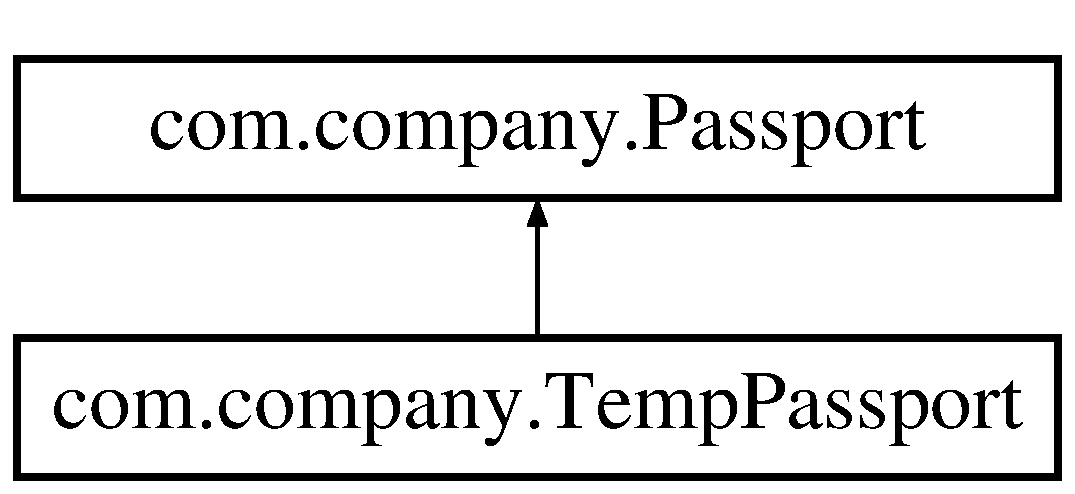
\includegraphics[height=2.000000cm]{classcom_1_1company_1_1Passport}
\end{center}
\end{figure}
\subsection*{Public Member Functions}
\begin{DoxyCompactItemize}
\item 
\mbox{\hyperlink{classcom_1_1company_1_1Passport_ae896b9cc83f86a204e4908e90b760a6e}{Passport}} ()
\begin{DoxyCompactList}\small\item\em Конструктор \end{DoxyCompactList}\item 
String \mbox{[}$\,$\mbox{]} \mbox{\hyperlink{classcom_1_1company_1_1Passport_a13c307f5067950667804b5d2d1ecc5bf}{get\+Info}} (String id)
\begin{DoxyCompactList}\small\item\em Метод, возвращающий форматированные данные о гражданине. \end{DoxyCompactList}\end{DoxyCompactItemize}


\subsection{Constructor \& Destructor Documentation}
\mbox{\Hypertarget{classcom_1_1company_1_1Passport_ae896b9cc83f86a204e4908e90b760a6e}\label{classcom_1_1company_1_1Passport_ae896b9cc83f86a204e4908e90b760a6e}} 
\index{com\+::company\+::\+Passport@{com\+::company\+::\+Passport}!Passport@{Passport}}
\index{Passport@{Passport}!com\+::company\+::\+Passport@{com\+::company\+::\+Passport}}
\subsubsection{\texorpdfstring{Passport()}{Passport()}}
{\footnotesize\ttfamily com.\+company.\+Passport.\+Passport (\begin{DoxyParamCaption}{ }\end{DoxyParamCaption})\hspace{0.3cm}{\ttfamily [inline]}}



Конструктор 



\subsection{Member Function Documentation}
\mbox{\Hypertarget{classcom_1_1company_1_1Passport_a13c307f5067950667804b5d2d1ecc5bf}\label{classcom_1_1company_1_1Passport_a13c307f5067950667804b5d2d1ecc5bf}} 
\index{com\+::company\+::\+Passport@{com\+::company\+::\+Passport}!get\+Info@{get\+Info}}
\index{get\+Info@{get\+Info}!com\+::company\+::\+Passport@{com\+::company\+::\+Passport}}
\subsubsection{\texorpdfstring{get\+Info()}{getInfo()}}
{\footnotesize\ttfamily String \mbox{[}$\,$\mbox{]} com.\+company.\+Passport.\+get\+Info (\begin{DoxyParamCaption}\item[{String}]{id }\end{DoxyParamCaption})\hspace{0.3cm}{\ttfamily [inline]}}



Метод, возвращающий форматированные данные о гражданине. 

Данная функция делает выборку из базы данных по имени пользователя и возвращает структуру с информацией о нем. 
\begin{DoxyParams}{Parameters}
{\em id} & Серия и номер паспорта \\
\hline
\end{DoxyParams}
\begin{DoxyReturn}{Returns}
Массив данных 
\end{DoxyReturn}

\begin{DoxyExceptions}{Exceptions}
{\em Not\+Found\+Exception} & Бросается, если пользователь не найден \\
\hline
\end{DoxyExceptions}


The documentation for this class was generated from the following file\+:\begin{DoxyCompactItemize}
\item 
src/com/company/\mbox{\hyperlink{Passport_8java}{Passport.\+java}}\end{DoxyCompactItemize}

\hypertarget{classcom_1_1company_1_1Registry}{}\section{com.\+company.\+Registry Class Reference}
\label{classcom_1_1company_1_1Registry}\index{com.\+company.\+Registry@{com.\+company.\+Registry}}


The documentation for this class was generated from the following file\+:\begin{DoxyCompactItemize}
\item 
src/com/company/\mbox{\hyperlink{Registry_8java}{Registry.\+java}}\end{DoxyCompactItemize}

\hypertarget{classcom_1_1company_1_1TempPassport}{}\section{com.\+company.\+Temp\+Passport Class Reference}
\label{classcom_1_1company_1_1TempPassport}\index{com.\+company.\+Temp\+Passport@{com.\+company.\+Temp\+Passport}}
Inheritance diagram for com.\+company.\+Temp\+Passport\+:\begin{figure}[H]
\begin{center}
\leavevmode
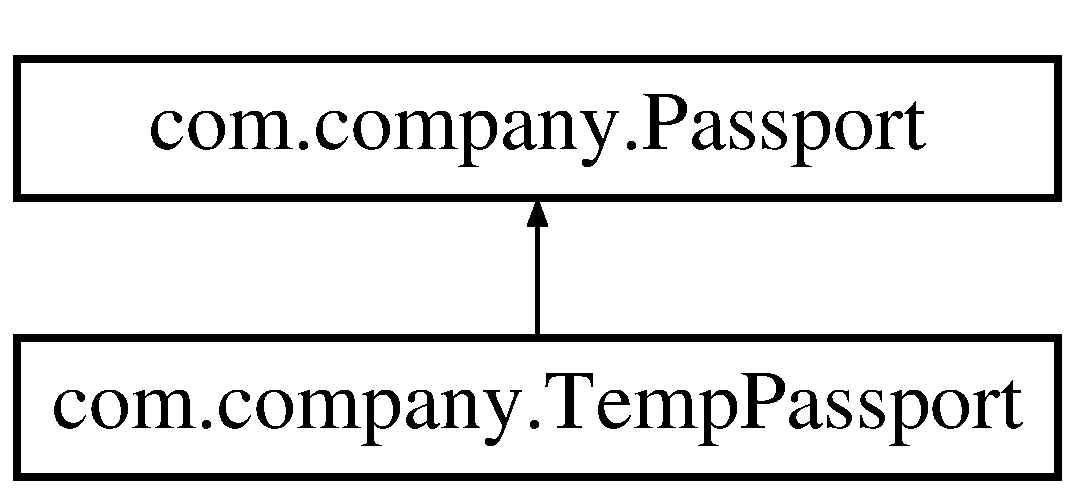
\includegraphics[height=2.000000cm]{classcom_1_1company_1_1TempPassport}
\end{center}
\end{figure}
\subsection*{Public Member Functions}
\begin{DoxyCompactItemize}
\item 
Date \mbox{\hyperlink{classcom_1_1company_1_1TempPassport_ae25b090b629cf145991f4f66d4d0ba86}{get\+Expired\+Date}} ()
\begin{DoxyCompactList}\small\item\em Геттер \end{DoxyCompactList}\item 
void \mbox{\hyperlink{classcom_1_1company_1_1TempPassport_ae72565902824ef39a74e4eb60d31e95e}{set\+Expired\+Date}} (Date expired\+Date)
\begin{DoxyCompactList}\small\item\em Сеттер \end{DoxyCompactList}\item 
Object \mbox{\hyperlink{classcom_1_1company_1_1TempPassport_ae107b7b36e00f9e677c410339622b261}{get\+Document}} (String name)
\begin{DoxyCompactList}\small\item\em Получить документ \end{DoxyCompactList}\end{DoxyCompactItemize}


\subsection{Member Function Documentation}
\mbox{\Hypertarget{classcom_1_1company_1_1TempPassport_ae107b7b36e00f9e677c410339622b261}\label{classcom_1_1company_1_1TempPassport_ae107b7b36e00f9e677c410339622b261}} 
\index{com\+::company\+::\+Temp\+Passport@{com\+::company\+::\+Temp\+Passport}!get\+Document@{get\+Document}}
\index{get\+Document@{get\+Document}!com\+::company\+::\+Temp\+Passport@{com\+::company\+::\+Temp\+Passport}}
\subsubsection{\texorpdfstring{get\+Document()}{getDocument()}}
{\footnotesize\ttfamily Object com.\+company.\+Temp\+Passport.\+get\+Document (\begin{DoxyParamCaption}\item[{String}]{name }\end{DoxyParamCaption})\hspace{0.3cm}{\ttfamily [inline]}}



Получить документ 

Дает данные о гражданине 
\begin{DoxyParams}{Parameters}
{\em name} & имя гражданина \\
\hline
\end{DoxyParams}
\begin{DoxyReturn}{Returns}
document 
\end{DoxyReturn}
\mbox{\Hypertarget{classcom_1_1company_1_1TempPassport_ae25b090b629cf145991f4f66d4d0ba86}\label{classcom_1_1company_1_1TempPassport_ae25b090b629cf145991f4f66d4d0ba86}} 
\index{com\+::company\+::\+Temp\+Passport@{com\+::company\+::\+Temp\+Passport}!get\+Expired\+Date@{get\+Expired\+Date}}
\index{get\+Expired\+Date@{get\+Expired\+Date}!com\+::company\+::\+Temp\+Passport@{com\+::company\+::\+Temp\+Passport}}
\subsubsection{\texorpdfstring{get\+Expired\+Date()}{getExpiredDate()}}
{\footnotesize\ttfamily Date com.\+company.\+Temp\+Passport.\+get\+Expired\+Date (\begin{DoxyParamCaption}{ }\end{DoxyParamCaption})\hspace{0.3cm}{\ttfamily [inline]}}



Геттер 

Возвращает дату окончания действия временного паспорта \begin{DoxyReturn}{Returns}
expired\+Date 
\end{DoxyReturn}
\mbox{\Hypertarget{classcom_1_1company_1_1TempPassport_ae72565902824ef39a74e4eb60d31e95e}\label{classcom_1_1company_1_1TempPassport_ae72565902824ef39a74e4eb60d31e95e}} 
\index{com\+::company\+::\+Temp\+Passport@{com\+::company\+::\+Temp\+Passport}!set\+Expired\+Date@{set\+Expired\+Date}}
\index{set\+Expired\+Date@{set\+Expired\+Date}!com\+::company\+::\+Temp\+Passport@{com\+::company\+::\+Temp\+Passport}}
\subsubsection{\texorpdfstring{set\+Expired\+Date()}{setExpiredDate()}}
{\footnotesize\ttfamily void com.\+company.\+Temp\+Passport.\+set\+Expired\+Date (\begin{DoxyParamCaption}\item[{Date}]{expired\+Date }\end{DoxyParamCaption})\hspace{0.3cm}{\ttfamily [inline]}}



Сеттер 

Изменяет дату окончания действия временного паспорта \begin{DoxyReturn}{Returns}
request 
\end{DoxyReturn}


The documentation for this class was generated from the following file\+:\begin{DoxyCompactItemize}
\item 
src/com/company/\mbox{\hyperlink{TempPassport_8java}{Temp\+Passport.\+java}}\end{DoxyCompactItemize}

\chapter{File Documentation}
\hypertarget{Guidance_8java}{}\section{src/com/company/\+Guidance.java File Reference}
\label{Guidance_8java}\index{src/com/company/\+Guidance.\+java@{src/com/company/\+Guidance.\+java}}


Седьмой вариант третьей лабораторной работы по ТРПО.  


\subsection*{Classes}
\begin{DoxyCompactItemize}
\item 
class \mbox{\hyperlink{classcom_1_1company_1_1Guidance}{com.\+company.\+Guidance}}
\end{DoxyCompactItemize}


\subsection{Detailed Description}
Седьмой вариант третьей лабораторной работы по ТРПО. 

Данный класс содержит реализацию работы АРМ руководства (просмотр статистики, поиск документов и заявок) \begin{DoxyAuthor}{Author}
Dementov 
\end{DoxyAuthor}
\begin{DoxyDate}{Date}
17.\+10.\+2017 
\end{DoxyDate}
\begin{DoxyVersion}{Version}
1.\+0 
\end{DoxyVersion}
\begin{DoxyParagraph}{Использует классы из пакета com.company\+:}
Passport Registry Maker 
\end{DoxyParagraph}
\begin{DoxyParagraph}{Использует зависимости\+: java.util.Array\+List}

\end{DoxyParagraph}

\hypertarget{Maker_8java}{}\section{src/com/company/\+Maker.java File Reference}
\label{Maker_8java}\index{src/com/company/\+Maker.\+java@{src/com/company/\+Maker.\+java}}


Седьмой вариант третьей лабораторной работы по ТРПО.  


\subsection*{Classes}
\begin{DoxyCompactItemize}
\item 
class \mbox{\hyperlink{classcom_1_1company_1_1Maker}{com.\+company.\+Maker}}
\end{DoxyCompactItemize}


\subsection{Detailed Description}
Седьмой вариант третьей лабораторной работы по ТРПО. 

Данный класс содержит реализацию работы АРМ изготовления паспортов (заказы, состояния, мастер печати)

\begin{DoxyAuthor}{Author}
Kharitonov 
\end{DoxyAuthor}
\begin{DoxyDate}{Date}
19.\+10.\+2017 
\end{DoxyDate}
\begin{DoxyVersion}{Version}
init 
\end{DoxyVersion}
\begin{DoxyParagraph}{Использует классы из пакета com.company\+:}
Passport 
\end{DoxyParagraph}
\begin{DoxyParagraph}{Использует зависимости\+: java.utils.Date, java.awt}

\end{DoxyParagraph}

\hypertarget{Passport_8java}{}\section{src/com/company/\+Passport.java File Reference}
\label{Passport_8java}\index{src/com/company/\+Passport.\+java@{src/com/company/\+Passport.\+java}}


Класс для хранения персональных данных гражданина  


\subsection*{Classes}
\begin{DoxyCompactItemize}
\item 
class \mbox{\hyperlink{classcom_1_1company_1_1Passport}{com.\+company.\+Passport}}
\end{DoxyCompactItemize}


\subsection{Detailed Description}
Класс для хранения персональных данных гражданина 

Содержит данные паспорта и осуществляет доступ к ним. \begin{DoxyAuthor}{Author}
Goi 

Dementov 

Kharitonov 
\end{DoxyAuthor}
\begin{DoxyDate}{Date}
15.\+10.\+2017 
\end{DoxyDate}
\begin{DoxyVersion}{Version}
init 
\end{DoxyVersion}

\hypertarget{Registry_8java}{}\section{src/com/company/\+Registry.java File Reference}
\label{Registry_8java}\index{src/com/company/\+Registry.\+java@{src/com/company/\+Registry.\+java}}


Седьмой вариант третьей лабораторной работы по ТРПО.  


\subsection*{Classes}
\begin{DoxyCompactItemize}
\item 
class \mbox{\hyperlink{classcom_1_1company_1_1Registry}{com.\+company.\+Registry}}
\end{DoxyCompactItemize}


\subsection{Detailed Description}
Седьмой вариант третьей лабораторной работы по ТРПО. 

Данный класс содержит реализацию работы АРМ приема и выдачи документов. \begin{DoxyAuthor}{Author}
Goi 
\end{DoxyAuthor}
\begin{DoxyDate}{Date}
16.\+10.\+2017 
\end{DoxyDate}
\begin{DoxyVersion}{Version}
1.\+0 
\end{DoxyVersion}
\begin{DoxyParagraph}{Использует классы из пакета com.company\+:}
Passport 
\end{DoxyParagraph}
\begin{DoxyParagraph}{Использует зависимости\+: java.utils.Date}

\end{DoxyParagraph}

\hypertarget{TempPassport_8java}{}\section{src/com/company/\+Temp\+Passport.java File Reference}
\label{TempPassport_8java}\index{src/com/company/\+Temp\+Passport.\+java@{src/com/company/\+Temp\+Passport.\+java}}


Класс для хранения персональных данных гражданина  


\subsection*{Classes}
\begin{DoxyCompactItemize}
\item 
class \mbox{\hyperlink{classcom_1_1company_1_1TempPassport}{com.\+company.\+Temp\+Passport}}
\end{DoxyCompactItemize}


\subsection{Detailed Description}
Класс для хранения персональных данных гражданина 

Содержит данные паспорта и осуществляет доступ к ним. \begin{DoxyAuthor}{Author}
Goi 
\end{DoxyAuthor}
\begin{DoxyDate}{Date}
19.\+10.\+2017 
\end{DoxyDate}
\begin{DoxyVersion}{Version}
1.\+1 
\end{DoxyVersion}

%--- End generated contents ---

% Index
\backmatter
\newpage
\phantomsection
\clearemptydoublepage
\addcontentsline{toc}{chapter}{Index}
\printindex

\end{document}
